% !TEX TS-program = pdflatex
% !TEX encoding = UTF-8 Unicode

% This is a simple template for a LaTeX document using the "article" class.
% See "book", "report", "letter" for other types of document.

\documentclass[11pt]{article} % use larger type; default would be 10pt

\usepackage[utf8]{inputenc} % set input encoding (not needed with XeLaTeX)

%%% Examples of Article customizations
% These packages are optional, depending whether you want the features they provide.
% See the LaTeX Companion or other references for full information.

%%% PAGE DIMENSIONS
\usepackage{geometry} % to change the page dimensions
\geometry{a4paper} % or letterpaper (US) or a5paper or....
% \geometry{margin=2in} % for example, change the margins to 2 inches all round
% \geometry{landscape} % set up the page for landscape
%   read geometry.pdf for detailed page layout information

\usepackage{graphicx} % support the \includegraphics command and options

% \usepackage[parfill]{parskip} % Activate to begin paragraphs with an empty line rather than an indent

%%% PACKAGES
\usepackage{booktabs} % for much better looking tables
\usepackage{array} % for better arrays (eg matrices) in maths
\usepackage{paralist} % very flexible & customisable lists (eg. enumerate/itemize, etc.)
\usepackage{verbatim} % adds environment for commenting out blocks of text & for better verbatim
\usepackage{subfig} % make it possible to include more than one captioned figure/table in a single float
% These packages are all incorporated in the memoir class to one degree or another...

%%% HEADERS & FOOTERS
\usepackage{fancyhdr} % This should be set AFTER setting up the page geometry
\pagestyle{fancy} % options: empty , plain , fancy
\renewcommand{\headrulewidth}{0pt} % customise the layout...
\lhead{}\chead{}\rhead{}
\lfoot{}\cfoot{\thepage}\rfoot{}

%%% SECTION TITLE APPEARANCE
\usepackage{sectsty}


\allsectionsfont{\sffamily\mdseries\upshape} % (See the fntguide.pdf for font help)
% (This matches ConTeXt defaults)

%%% ToC (table of contents) APPEARANCE
\usepackage[nottoc,notlof,notlot]{tocbibind} % Put the bibliography in the ToC
\usepackage[titles,subfigure]{tocloft} % Alter the style of the Table of Contents
\renewcommand{\cftsecfont}{\rmfamily\mdseries\upshape}
\renewcommand{\cftsecpagefont}{\rmfamily\mdseries\upshape} % No bold!

%%% END Article customizations


\usepackage[bulgarian]{babel}
\usepackage{physics}
\usepackage{amsmath}
\usepackage{centernot}
\usepackage{url}
\usepackage{graphicx}
\graphicspath{ {.} }
\usepackage{amsfonts}
\usepackage{xcolor}
\usepackage{enumitem}
\usepackage{systeme}
\usepackage{listings}
\usepackage[cache=false]{minted}
\usepackage{csquotes}
\setquotestyle{english}



%%% The "real" document content comes below...

\title{15. Модели на разпределени софтуерни архитектури}
\author{Play4u}
%\date{} % Activate to display a given date or no date (if empty),
         % otherwise the current date is printed
         

\newcommand{\lrangle}[1]{\left\langle #1 \right\rangle}

\newcommand{\oversetModels}[1]{\overset{#1}{\models}}

\newcommand{\italicBold}[1]{\textbf{\emph{#1}}}

\newcommand{\definition}{\italicBold{Дефиниция: }}
\newcommand{\theorem}{\italicBold{Теорема: }}
\newcommand{\lemma}{\italicBold{Лема: }}
\newcommand{\proof}{\italicBold{Доказателство: }}
\newcommand{\statement}{\italicBold{Твърдение: }}
\newcommand{\source}{\italicBold{Източник: }}

\newcommand{\integral}[4]{\displaystyle \int_{#1}^{#2}#3\,#4}

\newcommand{\redText}[1]{\textcolor{red}{#1}}

\newcommand{\curlies}[1]{\{#1\}}
\newcommand{\overbar}[1]{\mkern 1.5mu\overline{\mkern-1.5mu#1\mkern-1.5mu}\mkern 1.5mu}


\newcommand{\enumNum}{\renewcommand{\theenumi}{\arabic{enumi}}}
\newcommand{\enumlet}{\renewcommand{\theenumi}{\alph{enumi}}} 

\begin{document}
\maketitle

\italicBold{Конспект: } Изложението на въпроса трябва да включва следните по-съществени елементи:

\enumNum
\begin{enumerate}[noitemsep]
	\item Параметри на паралелната и разпределена обработка, метрика, методи за анализ
	\item Модели на разпределените софтуерни архитектури - процедурни, обектни, потокови, йерархични, асинхронни и интерактивни модели на софтуерната архитектура. Структури, организация, компоненти, приложение.
	\item Организация на разпределените приложения - клиент-сървър, двуслойни, трислойни и n-слойни модели. p2p. Сървъри за приложения и Web-сървъри. Метасистеми и грид. Сервизно-, моделно- и аспектно-ориентирани архитектури. Софтуерни агенти.
\end{enumerate}


\section{Паралелна и разпределена обработка}
\source Не успях да намеря много информация за тази част от темата. Мисля, че това е презентация \enquote{3. Конкурентно програмиране} от курса по РСА. Но даже и в презентацията няма чак толкова много информация по въпроса. Затова използвах източник \path{https://en.wikipedia.org/wiki/Analysis_of_parallel_algorithms} - би трябвало да върши работа.\\\par

За разлика от \enquote{нормалният}, асимптоматичен анализ на алгоритмите, който цели да намерим броя стъпки за изпълнението на един алгоритъм, анализът на паралелната и разпределена обработка има за цел да анализира как същият този алгоритъм би се представил при наличието на множество процесори. Така вторият анализ всъщност може да ни даде информация по какъв начин performence-а на нашия алгоритъм се променя спрямо броя на процесори, използвани за неговото изпълнение. Work-time(WT) framework-a, създаден от Shiloach и Vishkin се използва за извършването на този анализ.\\\par

Нека изчисленията се извършват на машина, която има $p$ процесора. Нека $T_{p}$ да е времето между началото и края на изчислителния процес. Анализът на на running time-a на алгоритъма се определя от следните входни параметри:
\begin{itemize}[noitemsep]
	\item \textit{Работата(work)}, извършена от $p$ процесори е общия брой примитивни операции които процесът изпълнява. Игнорирайки комуникационното забавяне от синхнронизацията на процесорите, работата е равна на времето за което се изпълнява алгоритъма на един процесор - означено чрез $T_{1}$.
	\item \textit{Дълбочината(depth или span)} е броя на най-дългата поредица от операции, които трябва да се извършат последователно поради \textit{data dependencies}. Дълбочината също може да се нарича \textit{критична дължина на критичния път} на алгоритъма. Минимизирането на дълбочината е важно когато създаваме паралелни алгоритми, тъй като дълбочината определя възможно най-краткото време за изпълнение. Също така, дълбочината може да бъде дефинирана като времето $T_{\infty}$, прекарано в изчисление, ако използваме идеална машина с безкраен брой процесори. 
	\item \textit{Цената(cost)} на изчислението е стойността $pT_{p}$. То представлява общото време прекарано, от всички процесори, в изчисление и изчакване.    
\end{itemize}  

Получаваме няколко полезни следствия от горните дефиниции:
\begin{itemize}[noitemsep]
	\item \textbf{Законът за работата(Work law)}. Цената винаги е най малко работата: $pT_{p}\geq T_{1}$. Това следва от факта, че $p$ процесора могат да извършат най-много $p$ операции паралелно.
	\item \textit{Законът за дълбочината(Span law)}. Краен брой $p$ процесора не могат да имат по добър performence от безкраен брой такива, и оттам $T_{p}\geq T_{\infty}$ 
\end{itemize}

Използвайки тези дефиниции и закони, можем да определим следните метрики на performence-a:
\begin{itemize}[noitemsep]
	\item \textit{Ускорението(speedup)} е увеличението на скоростта, получено от паралелното изпълнение в сравнение с последователното такова: $S_{p}=T_{1}/T_{p}$. Когато ускорението е $\Omega(n)$ за входни данни с размер $n$(използвайки Big O нотацията), ускорението е линейно, което е оптимално в прости модели на изчисление, тъй като от \textit{Законът за работата} следва, че $T_{1}/T_{p}\leq p$(на практика може да се получи т.нар. \textit{суперлинейно} ускорение, заради ефекти, породени от йерархията на паметта). Ако е изпълнено, че $T_{1}/T_{p}=p$, то тогава имаме т.нар. идеално линейно ускорение. Алгоритъм, който проявява линейно ускорение се нарича \textit{скалируем}.
	\item \textit{Ефикасността(Efficiency)} е ускорението за един процесор - $S_{p}/p$.
	\item \textit{Паралелизмът(Parallelism}) е съотношението $T_{1}/T_{\infty}$. То показва възможно най-голямото ускорение за всеки един брой процесори. От Закона за дълбочината, паралелизмът ограничава ускорението: ако $p > T_{1}/T_{\infty}$, тогава:\\
		\centerline{$\displaystyle \frac{T_{1}}{T_{p}}\leq \frac{T_{1}}{T_{\infty}} < p$.}
	\item \textit{Изоставането(Slackness)} е $T_{1}/(pT_{\infty})$. Изоставане по-малко от едно означава(от Закона за дълбочината), че идеалното линейно ускорение е невъзможно на $p$ процесора. 
\end{itemize}

Анализът на паралелните алгоритми обикновено се извършва с предположението, че разполагаме с неограничен брой процесори. Това не е релаистично, но не е и проблем, тъй като всяко едно изчисление което може да се извърши върху $N$ процесора, може да се извърши и върху $p < N$ процесора. Това е така, защото можем да накараме всеки дин процесор да извършва множество единици работа. В следствие от това се получава \textit{Законът на Брент}, който твърди че, една такава \enquote{симулация} може да се извърши за време $T_{p}$, ограничено по следния начин:\\
\centerline{$\displaystyle T_{p}\leq T_{N} + \frac{T_{1}-T_{N}}{p}$,}
или с по малка-точност,\\
\centerline{$\displaystyle T_{p}=O(T_{N}+\frac{T_{1}}{p})$.}
Алтернативен записване на горните и долни граници $T_{p}$ на закона е:\\
\centerline{$\displaystyle \frac{T_{1}}{p}\leq T_{p}\leq \frac{T_{1}}{p} + T_{\infty}$.}
Това показва, че дълбочината $T_{\infty}$ и работата $T_{1}$ заедно определят разумни граници на времето за изчисление. 
 
\section{Модели на разпределената софтуерна архитектура}
Моделирането на РСА е първата и най-важна фаза на проектиране, настройка, тестване, разгръщане и документация на разпределените среди за обслужване. Моделът на дадена софтуерна архитектура описва:
\begin{itemize}[noitemsep]
	\item Декомпозицията на процеса на компоненти
	\item Функционалната им композиция
	\item Прилаганият архитектурен стил - напр. процедурен, обектен, потоков(data flow), йерархичен или не-йерархичен, информационен(data centric), интерактивен(interaction oriented), базиран на изгледи(views) и др.
	\item Качествените (нефункционалните) атрибути на услугата - QoS
\end{itemize}

\subsection{Обектно-ориентиран}
Основните 4 принципа на ОО модела са:
\begin{itemize}[noitemsep]
	\item Енкапсулация - ограничаване на видимостта на функциите и прозрачността на имплементацията - вътрешен контекст и процедури - частни променливи в класовете, неустойчиви. Външен интерфейс - устойчив.
	\item Наследяване - адаптимост на кода чрез наследяване и допълване на спецификациите - т.е. от общо(родителски клас) към частно(наследен клас, дериват)
	\item Полиморфизъм - адаптивна функционалност чрез развитие на наследяването
	\item Абстракция - енкапсулация на данните с функциите върху тях; стандартни библиотеки от типове; публични и частни атрибути на типовете
\end{itemize}

Класовете са имплементации на абстрактни типове от данни, които се явяват техни \enquote{типове}. \\

Статични отношения между класовете:
\begin{enumerate}[noitemsep]
	\item конструкция на комплексни класове от класове
	\begin{enumerate}[noitemsep]
		\item композиция
		\item наследяване
	\end{enumerate}
	\item статична консистентност(т.е. логичност) на зависимите класове - като при базите данни
	\begin{enumerate}[noitemsep]
		\item агрегация
		\item асоциация\\
	\end{enumerate}
\end{enumerate}

Динамични отношения между класовете - обменът на съобщения\\
Обхват на ОО-архитектурите:\\

Предимства:
\begin{enumerate}[noitemsep]
	\item Непосредствена връзка с потребителските сценарии и проблемната област
	\item Преизползване(reuse) и капсулиране на имплементацията
	\item Лесно допълване чрез полиморфизма и класовете-деривати
	\item Устойчивост на системата поради защитеност на локалните атрибути
	\item Удобен преход към други модели и най-вече към компонентна архитектура\\
\end{enumerate}

Възможни проблеми:
\begin{enumerate}[noitemsep]
	\item Непредвидени странични ефекти при взаимодействието на много обекти, включително при асоциации 1...*
	\item Интерфейсите и вътрешната имплементация на класовете - макар и продукт на отделни фази - не са толкова разраничени, колкото при компонентните архитектури; обикновено се разработват съвместно, което снижава нивото на абстракция (и сложност) на цялата архитектура, а също обичайно води до по-финна гранулярност в сравнение с компонентните архитектури
	\item Наследствеността между класовете често води до грешки в спецификацията и следва да се прилаа много внимателно
\end{enumerate}

\subsection{Потокови(Data flow)}
Представят обработката като последователност от трансформации(т.е. групи операции) върху последователност от набори от стрктурирани еднотипни данни. Системата се декомпомозира на функционални модули и подисистеми - паралелизъм по управление - аналогия с нелинейните конвейери. Интерфейсът между модулите може да е във формата на потоци(стриймове), файлове, канали(pipes, асинхронни потоци) и др. Основният паралелизъм е по данни, тъй като ритъмът на обработка се задава от наличието на данни за обработка. По тази - отсъствие или минимизиране и импликация на контролния поток - ПА са подход и стил, приложим предимно при автоматизирани процеси на обслужване - напр. езикови компилатори, автоматизирани системи с пакетно обслужване като резпределените транзактивни систми, вградените системи\\\par
\textbf{Пакетна обработка}: Най-старият модел на СА за обслужване в транзактивни системи и класическите ОС със стандратен файлов IO и редиректори. Приложението е скрипт с команди за изпълнение на съответените модули в UNIX, DOS, Tcl/Tk-напр:
\begin{center}
	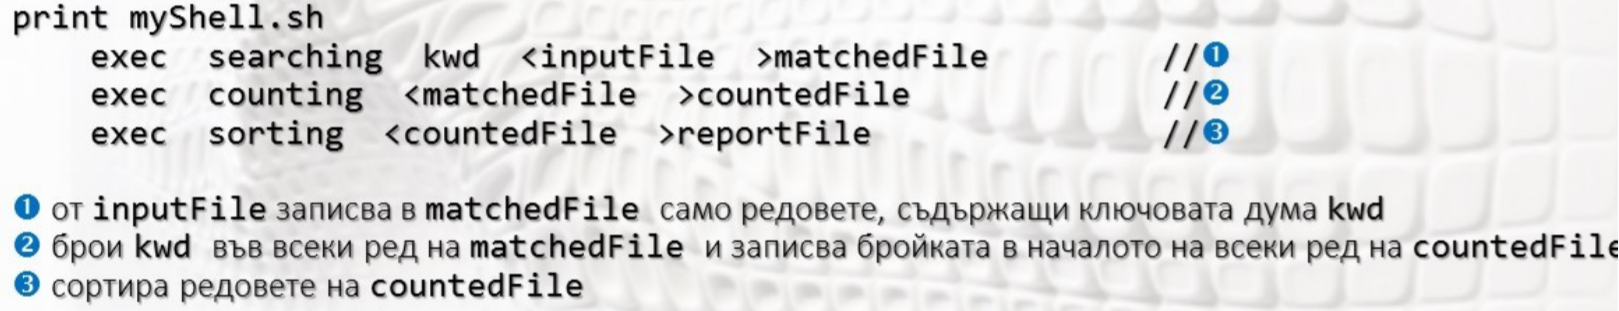
\includegraphics[scale=0.5]{PackageProcessing.png}
\end{center}
Този стил е приложим в съвременните ОО езици, където отделните обработващи модули, входът и изходът се представят като методи и атрибути на класа.\\
\textbf{Приложимост}
\begin{itemize}[noitemsep]
	\item Данните(вкл. междинните резултати) са оформени в пакети - файлове, т.е. с последователен достъп
	\item Модулите се представят като програми, които се активират със сркипт или като резидентни модули, които сканират входните си файлове
	\item Неприложими СА за интерактивен интерфейс
	\item Широко приложение за асинхронни паралелни процеси-данните се декомпозират като множество входни файлове, а обработващите модули се репликират в множество възли - принцип на обслужване в пакетната фонова обработка - Condor, Bonic, SETI@Home \\\par
\end{itemize}

\textbf{Филтрирани канали(Pipe \& Filter SA)}\\
Приложението се декомпозира на източник на данните, филтри, канали(pipes) и консуматор на данните(sink). Данните са последователни FIFO потоци(буфери, опашки) от байтове, символи или записи, които представят в последователен вид всички структури - вкл. и по-сложни, които се сериализират - в ОС marshalling/unmarshalling. Филтрите
\begin{itemize}[noitemsep]
	\item Трансформират потока данни - без необходимост да изчакват готовност на целия пакет за разлика от пакетната обработка
	\item Записват изходните данни в канал, който ги предава на друг асинхронно работещ филтър
	\item 2 типа филтри:
	\begin{itemize}[noitemsep]
		\item Активен филтър - изпълнява операциите pull/push върху пасивни канали - каналите осигуряват съответните операции, а инициативата е на филтъра. В Java PipedReader класовете предоставят интерфейс на тези канали
		\item Пасивен филтър - предоставя push/pull интерфейси на каналите\\
	\end{itemize}
\end{itemize}
Каналите преместват - а по същество съхраняват - потока данни, които се обменят между два филтъра

\subsection{Контекстни(Data centric)}
Характеризират се с централизирано хранилище на данните, които са достъпни за всички компоненти на системата, така че декомпозицията е на модул за управление на достъпа до данните и агенти, които извършват операции върху тях. Интерфейсът между агентите и данните може да е явен - напр. RMI или RPC - или имплиците - напр. транзактивен. В чист вид КАрх не предвиждат преки комуникации между информационните агенти. Модулът данни изпълнява операции по извличане или регистриране и промяна на записи - по 2 възможни модела:
\begin{itemize}[noitemsep]
	\item \textbf{Хранилище(repository)} - с активни(инициативни) агенти - хранилището е обикновенно оргранизирано като СУБД, CORBA, UDDI или Web-услуги
	\item \textbf{Черна дъска} - с инициатива на модула данни - агентите са абонати на събития(event listeners), които настъпват при промяна в данните и на които абонатите отговарят реактивно - често пр AI-разпределени приложения, охранителни системи за разпознаване на звук и образ, системи за управление на бизнес ресурси - складове, транспорт\\par
\end{itemize}

\textbf{Repository}\\
Макар и с управление по данни - за разлика от потоковите архитектури за пакетно обслужване на транзакции - тези архитектури поддържат интерактивните [U]I. Релационните СУБД са обичайната платформа за имплементация на тези архитектури, тъй като поддържат свъзаност (консистентност) на рпазпределения достъп до данните, както и множество системно средства за операции, базирани на метаданни. За по-висока отказоустойчивост и защита на данните се прилагат разпределени хранилища. \textbf{Основен недостатък} е статичната структура на данните - еволюция в структурата на релационните таблици се прилага трудно, струва скъпо и надежността й се проверява трудно.\\\par

\textbf{Черна дъска}\\
Ориентирани са главно към проблеми, решими с методите на AI - най-вече разпознаване на шаблони в различни области(първите приложения от края на 1970те са експертни системи в метеорология, изображения, свук, молекулярна химия). Те декомпозират решаването на проблеми също на два+ дяла:
\begin{itemize}[noitemsep]
	\item \textbf{Черна дъска}, съхраняваща данни - факти и хипотези, т.е. еволюционни можедли над фактите
	\item \textbf{Източници на знания} - паралелно работещи агенти, които съхраняват различни страни(данни, организирани като знания) от проблемната област - всеки ИЗ капсулира спеифичен аспект от проблема и е отговорен за частни хипотези и решения като част от общото решение
	\item (\textbf{Контролер} - система за начално зареждане и управление на разпределеното приложение)
\end{itemize}

Контролният поток е само от Черната дъска към ИЗточниците на знания:
\begin{itemize}[noitemsep]
	\item Неявни(имплицитни) обръщения към регистрираните в ЧД агенти-източници
	\item Обръщенията възникват при промени в данните и се предават към абонираните за тези промени ИЗ, които изпълняват реактивно заложените в тях логическо правила за извод
	\item Този асиметричен механизъм на обмен е известен като модел publish/subscribe(pub/sub) в общите комуникации 
	\item Класифицират се като слабо-свързана(loosely-coupled)PC поради асинхронния комуникационен модел с обмен на публикувани съобщения към абонатите (за разлика от силно-свързаните (tightly coupled) системи с хранилища, където транзитивното обслужване е свързано със заключване на данните за конкурентен достъп.)\\\par
\end{itemize}

\textbf{Обхват на КАрх с черна дъска}\\
Подходяща архитектура за комплексни неизследвани и особено мултидисциплинарни проблеми, които са:
\begin{itemize}[noitemsep]
	\item Без детерминистично решение с рпедставяне на контекста във формата на AI
	\item Неподходящи за търсене на решение с пълно обхождане на проблемния домейн поради изчислителна сложност или непълнотаюнеточност в данните.
\end{itemize}
Може да се генерират оптимално или няколко субоптимални решения или решения на частни подпроблеми; За разпределена обработка с умерена скалируемост поради централизирания контекст; Проблем е еволюцията в структурата на контекста поради обвързаност с агентите на знания; Отсъствието на междуагентни комуникации води до необходимост от централизирата им синхронизация(например приоритетна) на достъпа до общия контекст; Трудно се формулира условие за край на обработката поради недетрминистичния характер на проблемите

\subsection{Йерархични}
Декомпозират системата по управление на йерархични модули - т.е. функциите се групират по йерархичен принцип на няколко нива. Координацията обикновено е между модули от различни нива(вртикална свързаност) и се базира на явни (т.е. \enquote{заявка-отговор}) обръщения. Ниските нива функционират като услуги към непосредствените по-високи нива; услугите се имплементират като функции и процедури или пакети от класове. Пълна прозрачност между нивата се постига при запазване на свързващите интерфейси, но имплементацията на услугите може да еволюира. Архитектурен модел на ОС(Unix, MS. Net) и на протоколните стекове(TCP/IP); разслояване
\begin{itemize}[noitemsep]
	\item \textbf{Базови услуги} - системните услуги се групират в модули за IO, транзакции, балансирано планиране на процеси, защита на информацията
	\item \textbf{Междинен слой} - \enquote{ядро} - поддържа проблемно-ориентираната логика - бизнес приложения, числова обработка, информационна обработка, като представя интерфейси към колекции от базовите услуги
	\item \textbf{Потребителски интерфейсен слой} - напр. команден екран, графични контролни прозорци, Shell скрипт интепретатор
\end{itemize}

\subsection{Процедурни}
\textbf{Йерархия с подпрограми(Процедурни?):} Традиционна архитектура, предхожда ОО, базира се на процедури със споделен достъп на до данните (само частична енкапсулация). Декомпозицията е по управление, като комплексната функционалност на приложението се разделя на по-малки функционални групи - процедури и подпрограми - с цел тяхното споделяне между различните извикващи ги модули. Актуалните данни са параметри на обръщенията към изпълнителните функции и могат да се адресират по:
\begin{itemize}[noitemsep]
	\item Указател - подпрогамата може да променя техните стойности на същия адрес
	\item Стойност - подпрограмата получава стойностите като константи
	\item Име - подпрограмата използва като аргумент локалната стойност за съответното име - най-често това са локални имплементации на протоколи и други резидентни програми или динамични библиотеки
\end{itemize}
Главната програма управлява процеса на последователни обръщения към подпрограмите. Подпрограмите формират нефиксирана, но ациклична слоеста йерархия.\\\par

\textbf{Обхват на подпрограмните архитектури}\\
\begin{itemize}[noitemsep]
	\item Широко приложими при разделяне на функциите по принципа отгоре-надолу
	\item Приложими са и при ОО имплементация
	\item Проблем може да бъде достъпа до глобалните данни
	\item Глобалните данни са модел на (разпределена) обща памет - затова са по-подходящи при мултипроцесорни машини или имитиращите ги платформи MPSV - и обикновени аргументите на обрущението са указатели, а не стойности
\end{itemize}

\subsection{Асинхрнонни}
Базират се на неявни (имплицитни) асинхронни обръщения между обслужващите процеси. Асинхронният обмен може да бъде:
\begin{itemize}[noitemsep]
	\item Свързан(online) - \textit{без буфериране} - и двата процеса трябва да са активни, но не блокират изчакващото в точката на обмен
	\item Независим(offline) - \textit{с опосредяващ обмена процес-буфер} на съобщенията; приемащият процес може да не е активен в момента на изпращане на съобщенията и обратно
\end{itemize}
Активният процес генерира съобщенията, а пасивните проецси ги получават и евентуално изпълняват реакция
\begin{itemize}[noitemsep]
	\item Прилагат SW-шаблоните \textbf{Производител/Консуматор} или \textbf{ИЗдател/Абонат} $\equiv$ Наблюдател (Publisher/Subscriber, Observer)
	\item Управлението е по събитие(event-driven) - където събитието е издаване на съобщение от издателя и получаване на съобщение от абоната
\end{itemize}
В независимия вариант процесът-буфер алтернативно може да служи като:
\begin{itemize}[noitemsep]
	\item Централизатор \textbf{Message topic} на всички издадени съобщения и да ги препраща тематично до абонатите - един-към-много обмен
	\item Резервирана опашка \textbf{Message Queue} за един-към-един обмен\par
\end{itemize}

\textbf{Небуферирани асинхронни СА}\\
Системата за декомпозира на 2+ части
\begin{itemize}[noitemsep]
	\item Генератори на събития(sources)
	\item Слушатели на събития(event listeners)
	\item Регистратори на събития, които опосредяват обмена и по-конкретно поддържат асинхроността и неявното(непряко) оповестяване на слушателите
\end{itemize}

\textbf{Архитектурен модел на SmallTalk приложенията}: $n$ пасивни графични компонента-слушатели View\textsubscript{n} се регистрират в активно (т.е. инициативно) пространство на събития EventSpace за съобщения от даден генератор на събития Model\\\par

\textbf{Буферирани асинхронни СА}\\
Системата е:
\begin{itemize}[noitemsep]
	\item Контекстна(data-centric)
	\item Слабо-свързана(не се чака потвърждение за получаването на съобщенията и обикновено не се получава отговор след обработката) - но с надежден обем
	\item декомпозира се на 3 части
	\begin{itemize}[noitemsep]
		\item Генератори на съобщения(producers)
		\item Консуматори на съобщения
		\item Услуга за асинхронен буфериран обмен на съобщения - MOM(Message-Oriented Middleware)
	\end{itemize}
\end{itemize}
Висока скалируемост, надежност, p2p и CS приложения. Подходяща за системна поддръжка(мрежи, телекомуникация), бизнес приложения(бюлетини - новини, метеорология, групи по интереси; транзактивно банкиране и е-търговиря). Поддържа опашки (Message queuing, MQ) и тематичен обмен(Message Topic, Publish/Subscribe Messaging P\&S). Атрибути на съобщенията са ID, заглавие(header) и тяло. Клиентите на системата обменят съобщения инициативно или пасивно, като адресацията е на базата на идентификатор, получен при началната регистрация на клиента в услугата за обмен.\\\par

\textbf{Обхват на асинхронние СА}\\
Плюсове:
\begin{itemize}[noitemsep]
	\item Подходящи са за слабосвързани системи с устойчив неявен обмен на съобщения, при които обменящите процеси са анонимни - не знаят идентичността на комплементарния процес/и (в т.ч. и неговия интерфейс) - т.е. времева и локационна независимост
	\item Висока скалируемост и заменимост на компонентите
	\item Подходящ за динамично настройваеми разпределени изчисления(при асинхронен алгоритъм)
	\item Подходящи СА за пакетна обработка
	\item Подходящи за интегриране на наследени приложения (legacy systems) в съвременните проекти
\end{itemize}
Минуси:
\begin{itemize}[noitemsep]
	\item Независимостта между обменящите клиенти ограничава логиката на приложенията:
	\begin{itemize}[noitemsep]
		\item Логиката на клиентите трябва да е независима от получаването (и неполучаването) на конкретни съобщения
		\item Не се идентифицира източника и няма пряк обмен с него
	\end{itemize}
	\item Усложнена логика на клиентите поради изискването за гъвкавост т.е. всеки клиент се самоконтролира (котраст с йерархичните и централизираните системи)
	\item Възможност за тясно място(bottleneck) - по време(производителност на опашката/бюлетина) и по пространство (размер на опашката/бюлетина)
\end{itemize}

\subsection{Интерактивни}
Поддържат интензивен потребителски интерфейс. За целта декомпозицията на системата е на 3 функционални модула.
\begin{itemize}[noitemsep]
	\item Модул за представяне (изглед) - с потребителски интерфейс - за представяне (в т.ч.(това число) графично или мултимедийно) на изходните данни и също намеса на потребителите в обработката (т.е. вход за данни и контрол)
	\item Модул данни - поддържане на данните с базове функционалност върху тях
	\item Модул за управление - системни комуникации на процесите, инициализиране и конфигуриране на модулни данни, управление на изгледи
\end{itemize}
Поддържа множество (и то адаптивни) изгледи за даден набор данни. Слабо свързана архитектура, която поддържа явни и също обръщения към метод - респ, RMI и модел регистрация/уведомление (notification). Две категории ИСА:РАС(Presentation-Abstraction-Control) и MVC(Model-View-Controller)
\begin{itemize}[noitemsep]
	\item Аналогията е P-V, A-M и C-C
	\item Прилагат различно управление:
	\begin{itemize}[noitemsep]
		\item PAC е йерархично (разслоено) и разпределено управление, при което системата се формира от набор коопериращи агенти на три нива - базово ниво на общи данни и безнес логика, ниво на изгледите за локални данни и средни ниво агенти координатори на изгледите; всеки агент интегрира P, A и C компоненти
		\item В MVC агентите са равнопоставени
	\end{itemize}
\end{itemize}

\textbf{Обхват на MVC:} Това е базовата архитектура за приложения с интензивен потребителски I/O и динамично представяне на данните с възможност за самостоятелна имплементация на модулите. Поддържа се от множество професионални платформи за шаблонно развитие на приложенията. Не поддържа агентно-базиран информационен обмен, характерен за системите с редуциран птребителски интерфейс - автономни вградени системи, роботи, автонавигатори и др.\\\par

\textbf{Обхват на PAC:} Прилагат се за интерактивни системи от коопериращи специализирани информационни агенти. Слабосвързана разпределена система - комуникациите са неблокиращи и асинхронни.\\
Плюсове:
\begin{itemize}[noitemsep]
	\item Добри възможности за заменимост, еволюция на агентите, скалиране на системата
	\item Поддържа еднакво многонишкови и многопроцесни разпределени приложения 
\end{itemize}
Минуси:
\begin{itemize}[noitemsep]
	\item Значителен свръхтовар, особено при груповите комуникации
	\item Непряк (бавен) обмен между контекста и представянето му
	\item Имплементацията на A и P е зависима от тази на C - затруднение при проектирането
	\item Усложнени операции за отркиване на броя с идентифициране на текущите агенти
\end{itemize}
\end{document}






